\documentclass[12pt]{article}
\usepackage[utf8]{inputenc}
\usepackage[T1]{fontenc}
\usepackage[polish]{babel}
\usepackage{geometry}
\usepackage{tabularx}
\usepackage[table,xcdraw,dvipsnames]{xcolor}
\usepackage{color}
\usepackage{subfig}
\usepackage{sidecap}
\usepackage{wrapfig}
\usepackage{float}
\usepackage{enumerate}
\usepackage{graphicx}
\usepackage{multirow}
\usepackage{hyperref}
\usepackage{titlesec}
\usepackage{amsmath}
\usepackage{anyfontsize}
\usepackage{indentfirst}
\usepackage{listings}
\usepackage{multicol}
\usepackage{pgfplots}
\usepackage{fancyhdr}

\newgeometry{tmargin=1.8cm,bmargin=1.8cm,lmargin =1.8cm,rmargin=1.8cm}

\begin{document}
\begin{titlepage}
\begin{figure}
    \centering
    
\includegraphics[width=18cm]{logo-PWr.png}
    \label{fig:pwr}
\end{figure}
    \begin{center}
        \LARGE \textbf{ Wydział Elektroniki, Fotoniki i Mikrosystemów }\\ 
        \vspace{70pt}
        \Huge \textit{ Sterowanie Procesami Ciągłymi}  \\
    \end{center}
    \vspace{30pt}
    \hrule
    \vspace{1pt}
    \hrule
    \begin{center}
        {\fontsize{30}{50}\selectfont Sprawozdanie nr 1\\ }
        \vspace{10pt}
        {\fontsize{25}{25}\selectfont Charakterystyki czasowe  }
    \end{center}
    \hrule
    \vspace{1pt}
    \hrule
    \begin{flushright}
        \vspace{50pt}

        \textit{\Large Prowadzący:}\\
        \Large dr hab. inż. Grzegorz Mzyk\\
        \vspace{10pt}
        \textit{\Large Wykonała:}\\
        \Large Zuzanna Mejer, 259382 \\
        \vspace{10pt}
        \textit{\Large Termin zajęć:}\\
        \Large czwartek TP, 9:15\\
        \vspace{10pt}
    
    \end{flushright}
    \vspace{60pt}
    \begin{center}
        \large Wrocław, \today r.
    \end{center}
\end{titlepage}
    
    
\tableofcontents
\newpage

\section{Cel ćwiczenia}
Głównymi celami ćwiczenia było: zbadanie zależności odpowiedzi systemu w dziedzinie czasu od pulsacji pobudzenia sinusoidalnego; zapoznanie się z różnymi rodzajami charakterystyk częstotliwościowych oraz zbadanie wpływu wartości parametrów układu opóźniającego z inercją na charakterystykę częstotliwościową układu.


\section{Zależność charakterystyki czasowej układu od wartości pulsacji pobudzenia sinusoidalnego}
Badany jest asymptotycznie stabilny układ liniowy o zadanej transmitancji:
\begin{equation}
    K(s) = \frac{1}{s^2+0,1s+1},
    \label{transmitancja}
\end{equation}
który pobudzany jest sygnałem sinusoidalnym o ogólnym wzorze:

\begin{equation}
    u(t) = sin(\omega t),
\end{equation}
gdzie $\omega$ to pulsacja. Odpowiedź układu liniowego na pobudzenie sinusoidalne w stanie ustalonym ma postać:
\begin{equation}
    y_{ust}(t) = A \cdot sin(\omega t + \phi),
\end{equation}
gdzie: $A$ to amplituda, $\omega$ to pulsacja oraz $\phi$ to przesunięcie fazowe. Wiedząc, że pulsacja odpowiedzi systemu $\omega$ jest identyczna jak pulsacja sygnału wejściowego, zbadano jaka jest zależność między pulsacją sygnału wejściowego a amplitudą $A$ i przesunięciem fazowym $\phi$ odpowiedzi systemu. Do badań przyjęto 3 wartości pulsacji: $\omega = 0,1$, $\omega = 1$, $\omega = 10$, co oznacza, że układ o transmitancji \ref{transmitancja} pobudzono kolejno: $u_1(t) = sin(0,1t)$, $u_2(t) = sin(1t)$ oraz $u_3(t) = sin(10t)$.  Zbudowano następujący schemat w Simulinku:
\begin{figure}[H]
    \centering
    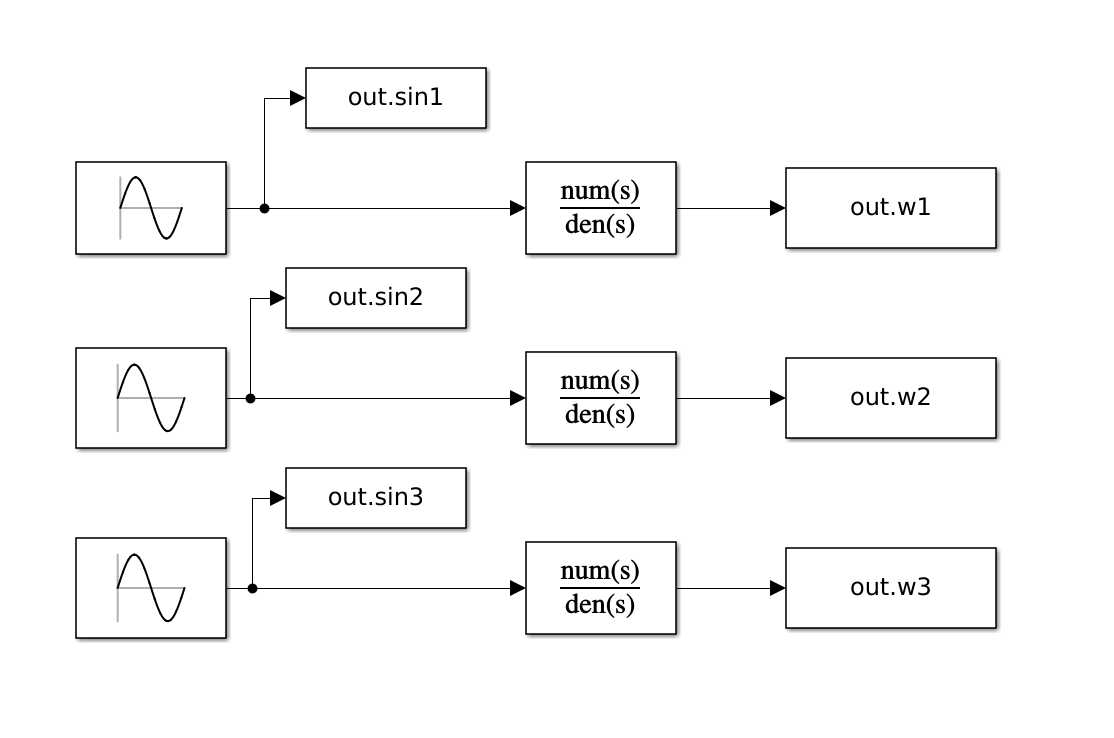
\includegraphics[scale=0.25]{2.png}
    \caption{Schemat w Simulinku do badania odpowiedzi układu na pobudzenie sinusoidalne}
\end{figure}


\subsection{Odpowiedź systemu na pobudzenie sinusoidalne, gdy pulsacja $\omega = 0,1$}
Pobudzono układ sygnałem $u_1(t)=sin(0,1 t)$. Poniżej przedstawiono porównanie pobudzenia sinusoidalnego (kolor czarny na wykresie) z odpowiedzią systemu (kolor czerwony na wykresie).
\begin{figure}[H]
    \centering
    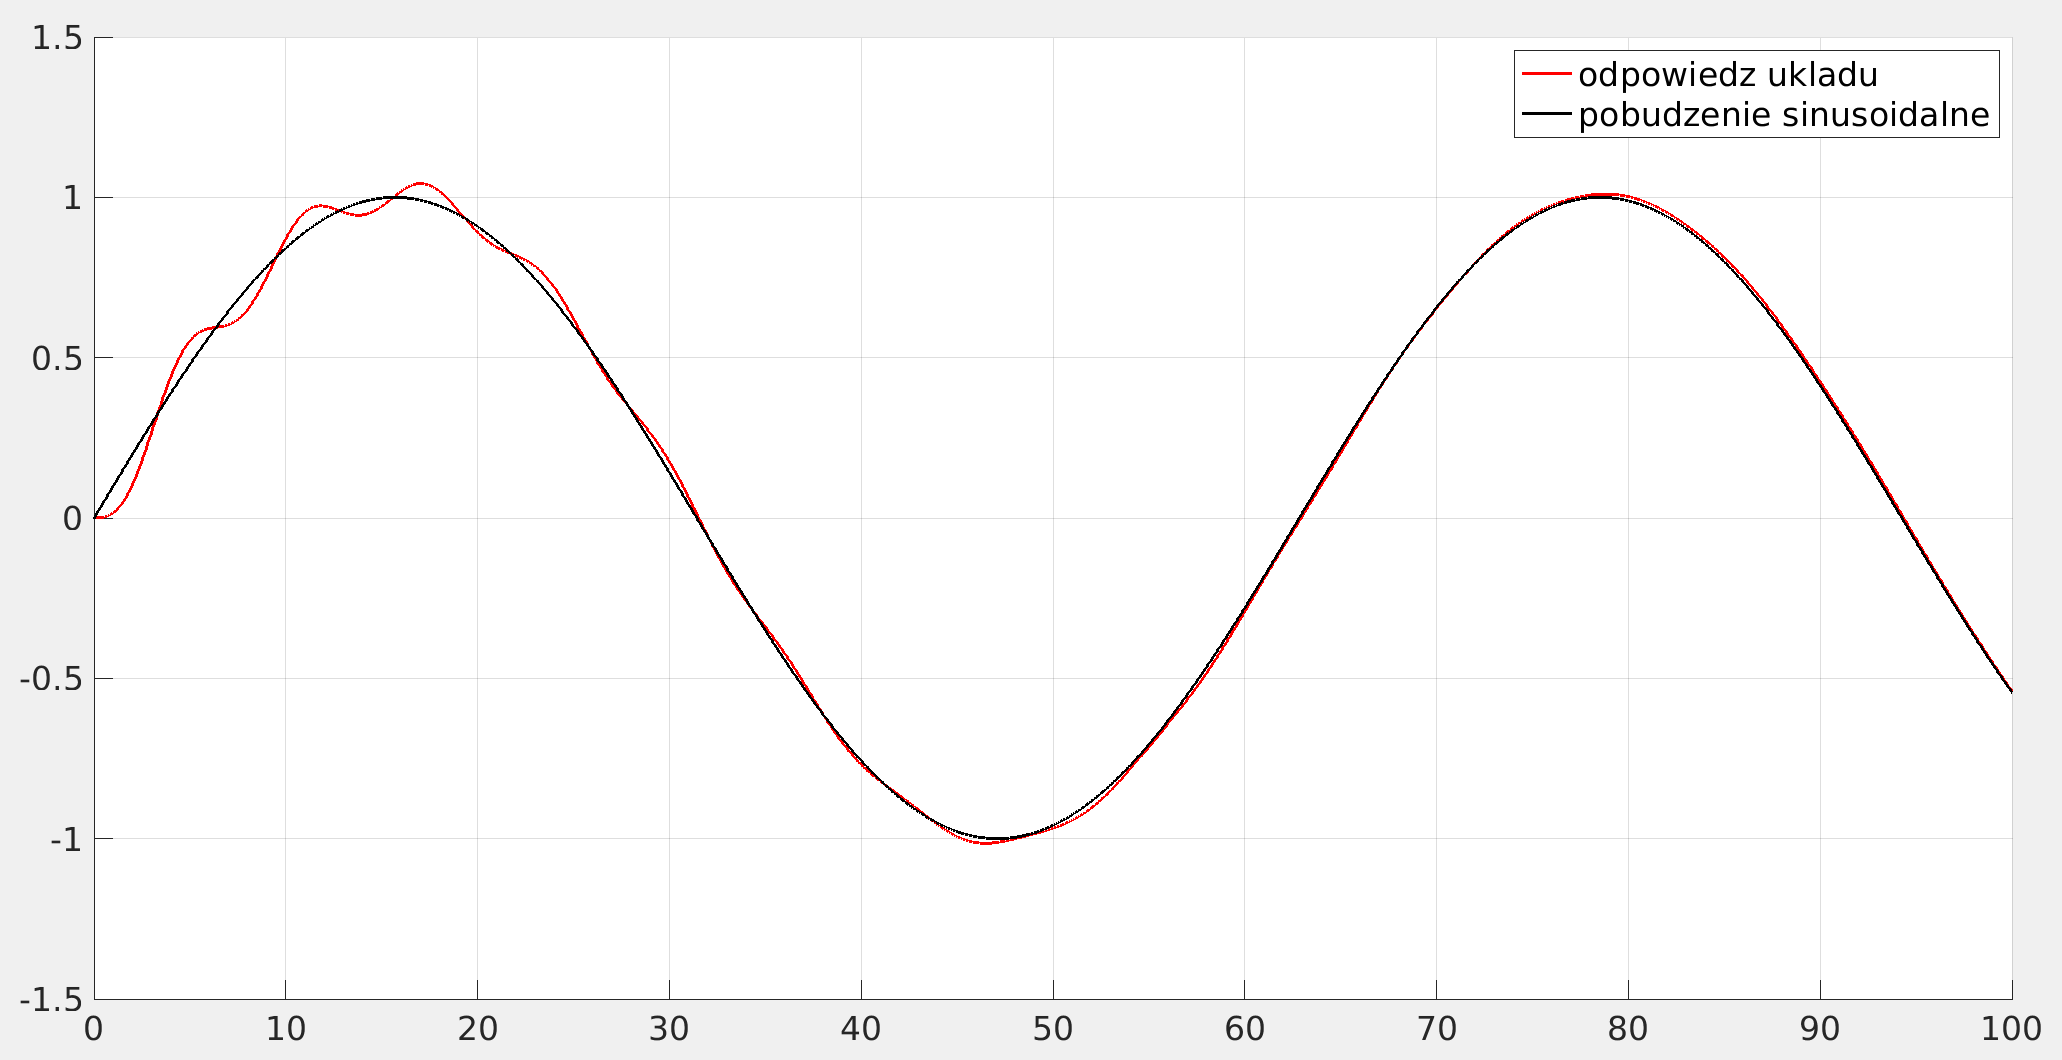
\includegraphics[scale=0.2]{2.1.png}
    \caption{Odpowiedź systemu o transmitancji K(s) na pobudzenie $u_1(t)=sin(0,1 t)$}
\end{figure}

\colorbox{Dandelion}{przesuniecie fazowe i amplituda; oznaczyc? opisac?}

\subsection{Odpowiedź systemu na pobudzenie sinusoidalne, gdy pulsacja $\omega = 1$}
Pobudzono układ sygnałem $u_2(t)=sin(1 t)$. Poniżej przedstawiono porównanie pobudzenia sinusoidalnego (kolor czarny na wykresie) z odpowiedzią systemu (kolor czerwony na wykresie).
\begin{figure}[H]
    \centering
    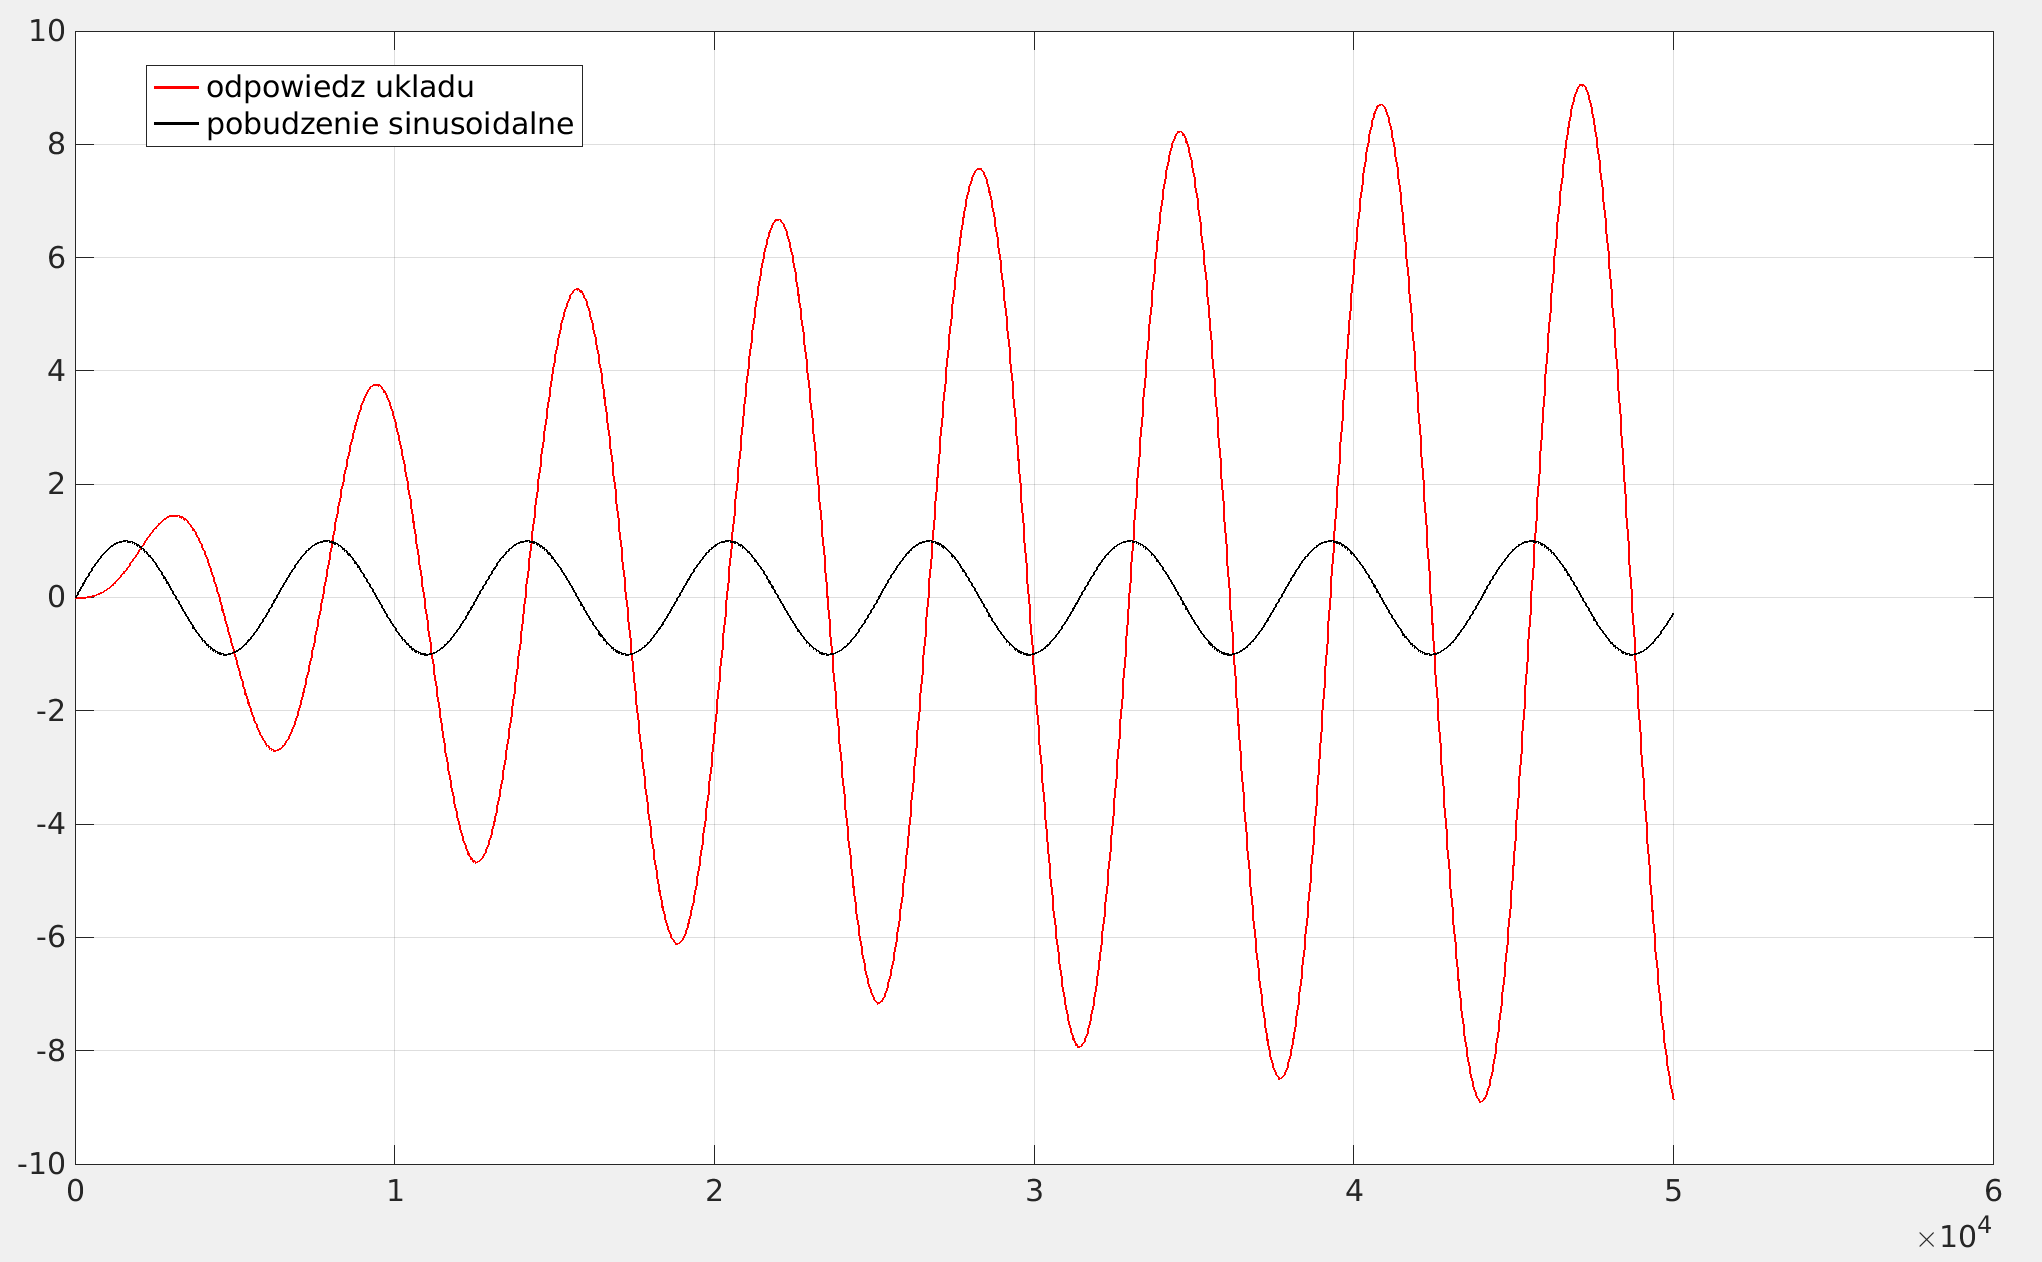
\includegraphics[scale=0.2]{2.2.png}
    \caption{Odpowiedź systemu o transmitancji K(s) na pobudzenie $u_2(t)=sin(1 t)$}
\end{figure}

\colorbox{Dandelion}{przesuniecie fazowe i amplituda; oznaczyc? opisac?}

\subsection{Odpowiedź systemu na pobudzenie sinusoidalne, gdy pulsacja $\omega = 10$}
Pobudzono układ sygnałem $u_3(t)=sin(10 t)$. Poniżej przedstawiono porównanie pobudzenia sinusoidalnego (kolor czarny na wykresie) z odpowiedzią systemu (kolor czerwony na wykresie).
\begin{figure}[H]
    \centering
    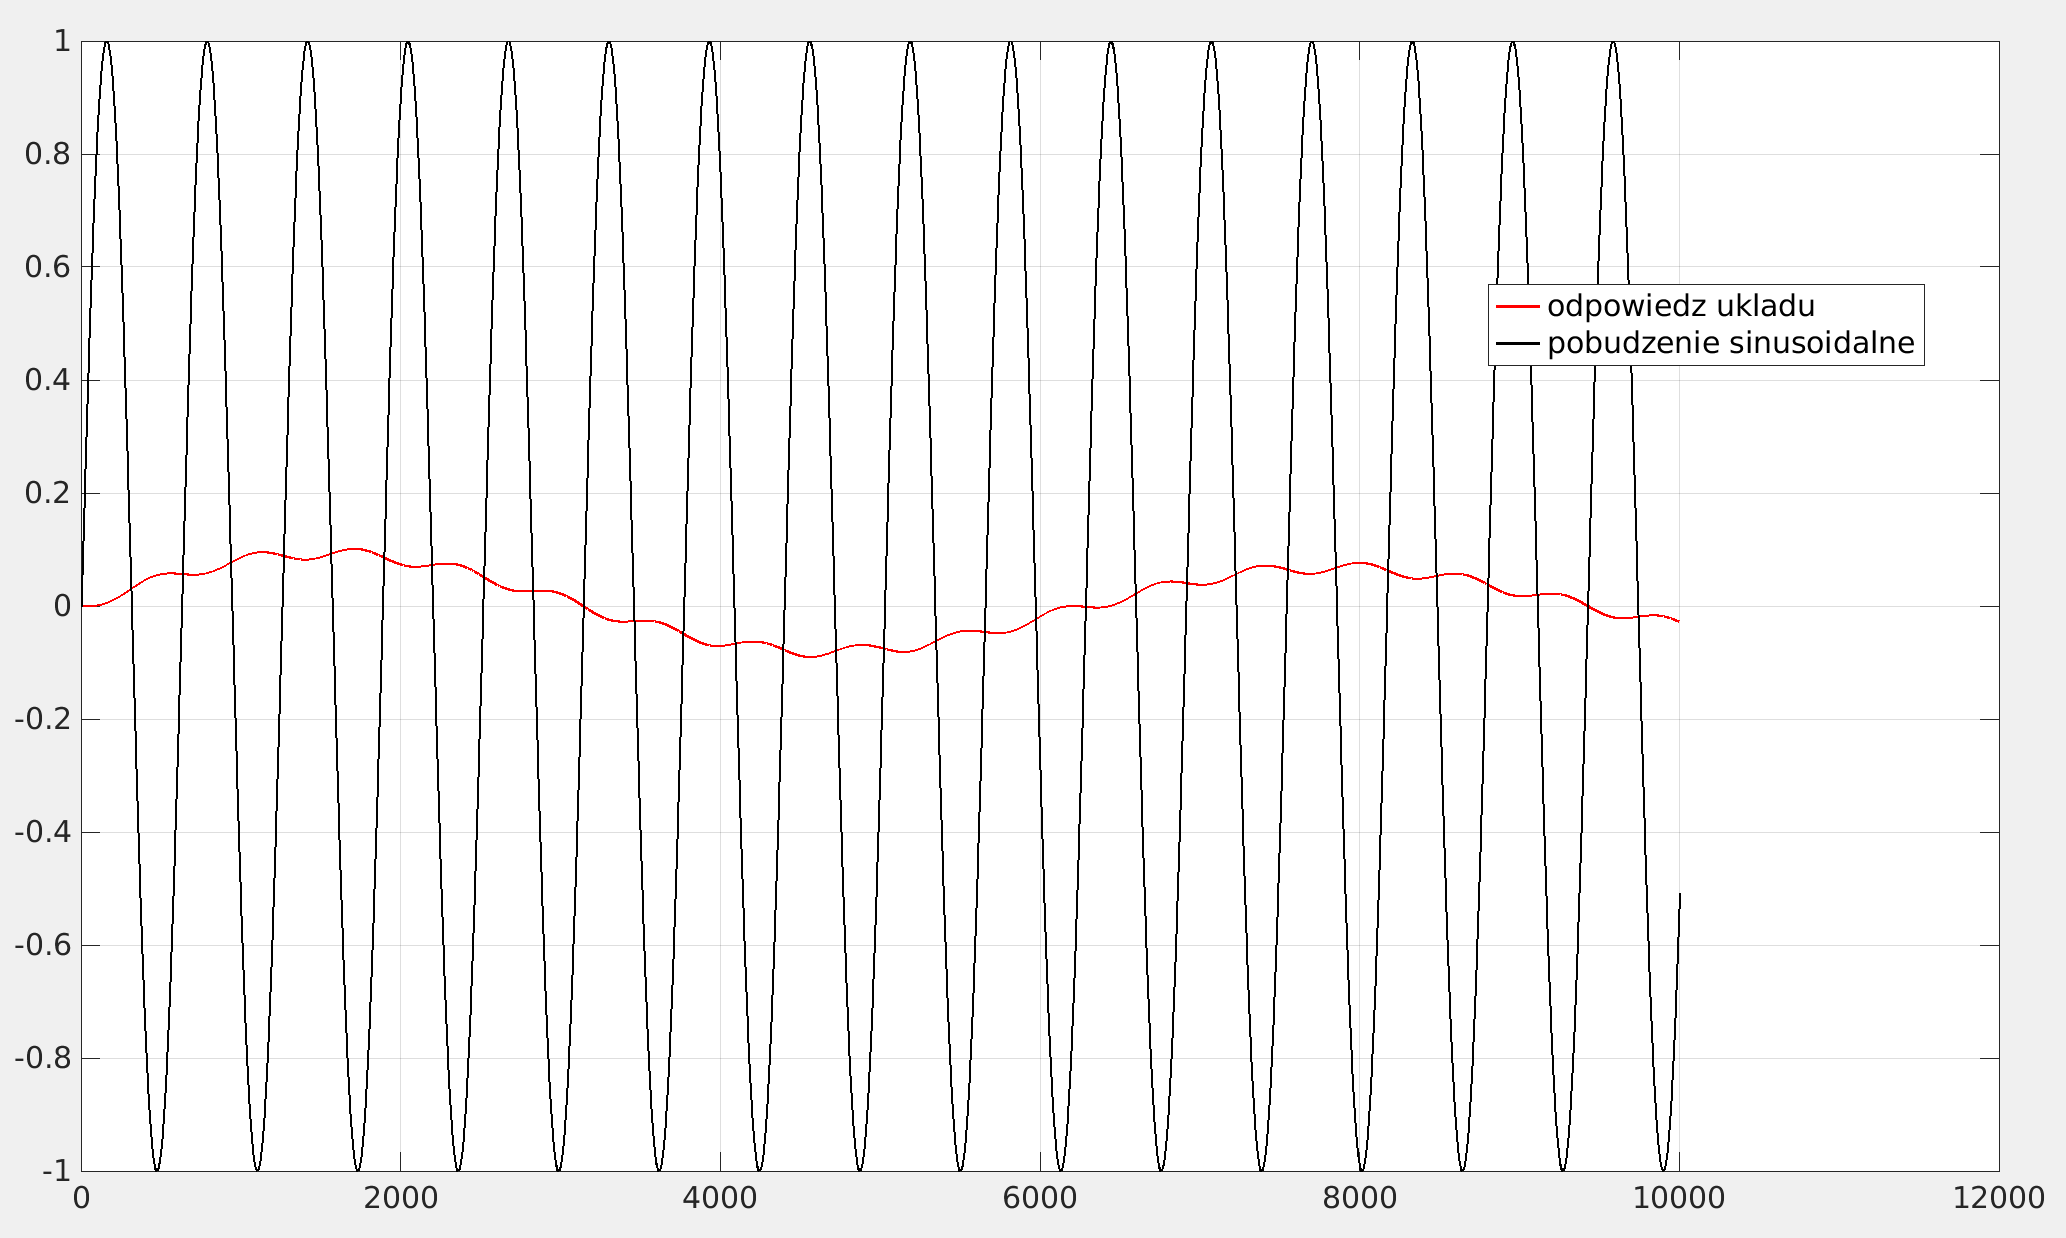
\includegraphics[scale=0.2]{2.3.png}
    \caption{Odpowiedź systemu o transmitancji K(s) na pobudzenie $u_3(t)=sin(10 t)$}
\end{figure}

\colorbox{Dandelion}{przesuniecie fazowe i amplituda; oznaczyc? opisac?}

\subsection{Porównanie}


% Wzmocnienie amplitudy A oraz wprowadzone przesunięcie fazowe
% φ są zale ̇zne od ω, odpowiednio
% A(ω) = STRONA 64

\section{Badania w dziedzinie częstotliwościowej}
\subsection{Charakterystyka amplitudowo-fazowa}
\subsection{Analiza charakterystyki częstotliwościowej układu opóźniającego z inercją}

\section{Podsumowanie i wnioski}

\end{document}